% !TeX encoding = UTF-8
% !TeX spellcheck = en_GB

%%% Add [final] option to the report class to switch between draft and final version of the report
%%% Use [narrowmargin] to enable narrow margins - this may impair readability.
%\documentclass[a4paper,12pt,draft]{include/intocpsreport}   %Or
\documentclass[a4paper,12pt,final]{include/intocpsassociation}   %Or
% intocpslargereport if chapters are required.
%
%
%
\usepackage[T1]{fontenc}
\usepackage[utf8]{inputenc}
\usepackage{longtable}
\usepackage{tikz-uml}
\usepackage{framed}
\usepackage{subcaption}
% \usepackage[hyphenbreaks]{breakurl}
\usepackage{xurl}
\usepackage{color}
\usepackage{amsmath}
\usepackage{courier}
\usepackage{xspace}
\usepackage{cleveref}
\usepackage{subcaption}
\usepackage{textcomp} % Used for 20-sim section \textrightarrow
%\usepackage{showframe}
\usepackage[section]{placeins}
\usepackage{listings}
\usepackage{glossaries}
\usepackage{MnSymbol}
%% Define listing environment for XML
\definecolor{gray}{rgb}{0.4,0.4,0.4}
\definecolor{darkblue}{rgb}{0.0,0.0,0.6}
\definecolor{cyan}{rgb}{0.0,0.6,0.6}

\lstset{
  basicstyle=\footnotesize\ttfamily,
  columns=fullflexible,
  showstringspaces=false,
  commentstyle=\color{gray}\upshape
}
\crefname{lstlisting}{Listing}{Listings}
\Crefname{lstlisting}{Listing}{Listings}
\lstdefinelanguage{XML}
{
  morestring=[b]",
  morestring=[s]{>}{<},
  morecomment=[s]{<?}{?>},
  stringstyle=\color{black},
  identifierstyle=\color{darkblue},
  keywordstyle=\color{cyan},
  morekeywords={xmlns,version,type}% list your attributes here
}

\colorlet{numb}{magenta!60!black}
\lstdefinelanguage{json}{
    basicstyle=\normalfont\ttfamily,
    stringstyle=\color{black}, % style of strings
      identifierstyle=\color{darkblue},
    showstringspaces=false,
    breaklines=true,
    string=[s]{"}{"},
    comment=[l]{:\ "},
    morecomment=[l]{:"},
    literate=
        *{0}{{{\color{numb}0}}}{1}
         {1}{{{\color{numb}1}}}{1}
         {2}{{{\color{numb}2}}}{1}
         {3}{{{\color{numb}3}}}{1}
         {4}{{{\color{numb}4}}}{1}
         {5}{{{\color{numb}5}}}{1}
         {6}{{{\color{numb}6}}}{1}
         {7}{{{\color{numb}7}}}{1}
         {8}{{{\color{numb}8}}}{1}
         {9}{{{\color{numb}9}}}{1}
}


\lstnewenvironment{xml}[1][]{\lstset{  language=XML,
  morekeywords={encoding, xs:schema,xs:element,xs:complexType,xs:sequence,xs:attribute}}\lstset{#1}}
{}

%% end listing environment for XML
%
%
%
\def\draftnote#1{\noindent\smallskip\framebox{\begin{minipage}{0.95\columnwidth}\color{red}#1\end{minipage}}\smallskip\par}
\newenvironment{draftnoteenv}{\noindent\smallskip\begin{framed}\begin{minipage}{0.95\columnwidth}\color{red}}{\end{minipage}\end{framed}\smallskip\par}
\newenvironment{assumption}{\noindent\smallskip\color{blue}\begin{framed}\begin{minipage}{0.95\columnwidth}}{\end{minipage}\end{framed}\smallskip\par}
%
%
%
\newcommand{\revisit}[1]{\textcolor{red}{\pmb{[[[}\@ #1\@ \pmb{]]]}}}
%
%
\reporttitle{INTO-CPS External Data Broker FMU\\\vspace{1em} (RabbitMQ FMU)}
\shortreporttitle{INTO-CPS EDB FMU}  %To use if report title is too long for header
%
%
%
%%% Set document release class as appropriate
%%% e.g. Public, Restricted, Programme Participant
\reportstatus{Public}
%
%
%
%%% If document is a deliverable, this flag should be commented out
%%% e.g. %\technotetrue
%%% If report is a technical report, leave uncommented
%%% e.g. \technotetrue
\technotetrue % Comment out as appropriate
%
%
%
\submissiondate{February 14, 2020}
\contributors{
Casper Thule, Aarhus University, Centre for Digital Twins \\
Kenneth Lausdahl, Mj{\o}lner Informatics A/S \\
Cl\'audio Gomes, Aarhus University, Centre for Digital Twins
}
%
%
%
\editors{
Casper Thule, Aarhus University, Centre for Digital Twins
}
%
%
%
%\reviewers{Ken Pierce, UNEW\\
%Kangfeng Ye, UY\\
%Luis Diogo Couto, UTRC}
%
%
%
%% Version details
% #1: version
% #2: date
% #3: author
% #4: description
\addversion{1.0}{January 23, 2020}{Casper Thule}{First version.}
\addversion{1.1}{February 14, 2020}{Casper Thule}{Updated with link to RabbitMQ
  FMU repository. Added extra information.}


%
%
\begin{document}
\maketitle
%
%
%
%%%% Document abstract page %%%%
\section*{Abstract}
\label{sec:abstract}
%
This document concerns an implementation of an External Data Broker (EDB) FMU based on
RabbitMQ. An EDB FMU brings external data into an FMI context by receiving data
external to the FMI simulation and make it available via FMI outputs. The
specific RabbitMQ based implementation is realised in RabbitMQ FMU.

Several of the constructs in the approach presented in this publication is general and can applied to multiple
cases. For example, the RabbitMQ FMU can be adapted to process different messages by
making changes to its static description file, without the need to recompile the
binaries, which are already compiled for Mac, Linux and Windows. Additionally, the implementation can be made to fit other message-oriented or
data-stream middlewares while still reusing most of the source.

As such, while RabbitMQ FMU is exemplified with a certain scenario, it can be applied generally and does not have a specific
scenario tied to it.

The actual implementation is available at: \url{https://github.com/INTO-CPS-Association/fmu-rabbitmq/releases}
%
\newpage
%
%%%% Document table of contents page %%%%
\tableofcontents
\newpage
%
%
%
%%%% Document Content %%%%
%% \chapter{Chapter Title} %% if intocpslargereport is in use
%\begin{assumption}
%
%
%
\section{Introduction}\label{sec:intro}
EDB is short for External Data Broker and EDB FMU is an FMU that brings external
data into an FMI context. The implementation of EDB FMU described in this
publication is based on RabbitMQ. However, this is just one way to implement an
EDB FMU. Several of the constructs described in this publication are general and
can be used with other message-oriented or data streaming middleware. For this
reason, both EDB FMU and RabbitMQ FMU will be used throughout this document,
where EDB FMU is generally applicable functionality, whereas RabbitMQ FMU is an
implementation of EDB FMU specific to RabbitMQ. Thus, one could take the
existing source code of RabbitMQ FMU and fit it to another middleware than
RabbitMQ while still reusing most of the source code.
Note, that this document assumes general knowledge of
the Functional Mock-up Interface (FMI)~\cite{FMIStandard2.1}.

An overall approach to using an EDB FMU in a digital twin context is depicted
in~\cref{fig:interfacing_overview}, where the content within the \textit{System Specific} frame will vary based on the system
providing the data. The Log-Translator entity translates the
system-specific log messages to digital twin compatible messages and publishes
them to a Data Middleware Node (i.e. a RabbitMQ Node). The EDB FMU is configured
via its static description to
receives messages from the Data Middleware Node. The message content is then
parsed and published via regular FMI outputs.

\begin{figure}[htb]
  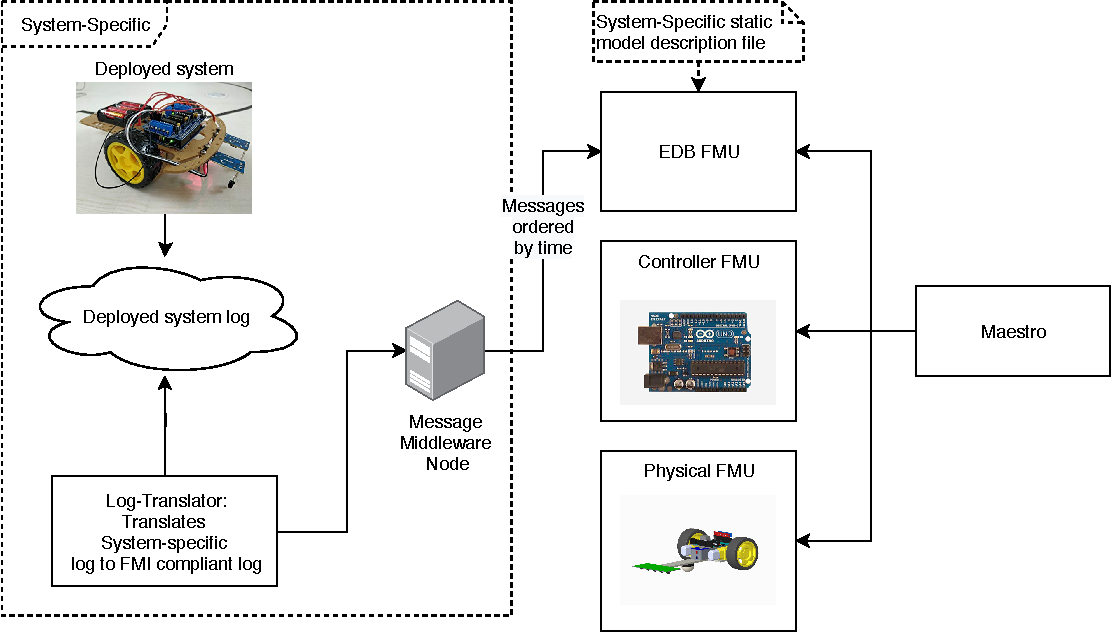
\includegraphics[width=\textwidth]{figures/overview.pdf}
  \caption{Interfacing Overview}
 \label{fig:interfacing_overview}
\end{figure}

This approach generalises the FMI enabling entity, the EDB FMU, such that
it can be used for different kinds of systems with different kinds of logging
facilities. The motivation behind this approach is that tools of the INTO-CPS Association
should be generally applicable.

The following chapters describes the following in order:
\begin{description}
  \item[Time Handling] How system-time and simulation time is mapped and put in
    an FMI simulation context.
  \item[Data Handling] How message content and the state of EDB FMU are
    coordinated.
  \item[Configuration] How to configure an EDB/RabbitMQ FMU via the ModelDescription File
  \item[Example - Single Water Tank RabbitMQ] This example demonstrates how RabbitMQ FMU
    acts as an External Data Broker in context of a Single Water Tank Digital Twin. It focuses solely on this part and does not
    contain a deployed system.

    \item[Example - Line Following Robot] IN PROGRESS - This example demonstrates transmission
    of data from a deployed line following robot. The data is made available in
    the FMI co-simulation via RabbitMQ FMU. Thus, this is a example with
    both a deployed system, its digital twin and the RabbitMQ FMU.
  \item[Future Work] Describes some ideas for future work.
\end{description}


%%% Local Variables:
%%% mode: latex
%%% TeX-master: "../rabbitmq-fmu"
%%% End:

\newpage
\section{Time Handling}\label{sec:time_handling}
This section concerns the digital twin and how data time is handled with
relation to FMI.
The description below is accompanied by \cref{fig:time-handling_simulation-view}.

\begin{figure}[!htb]
  \centering
  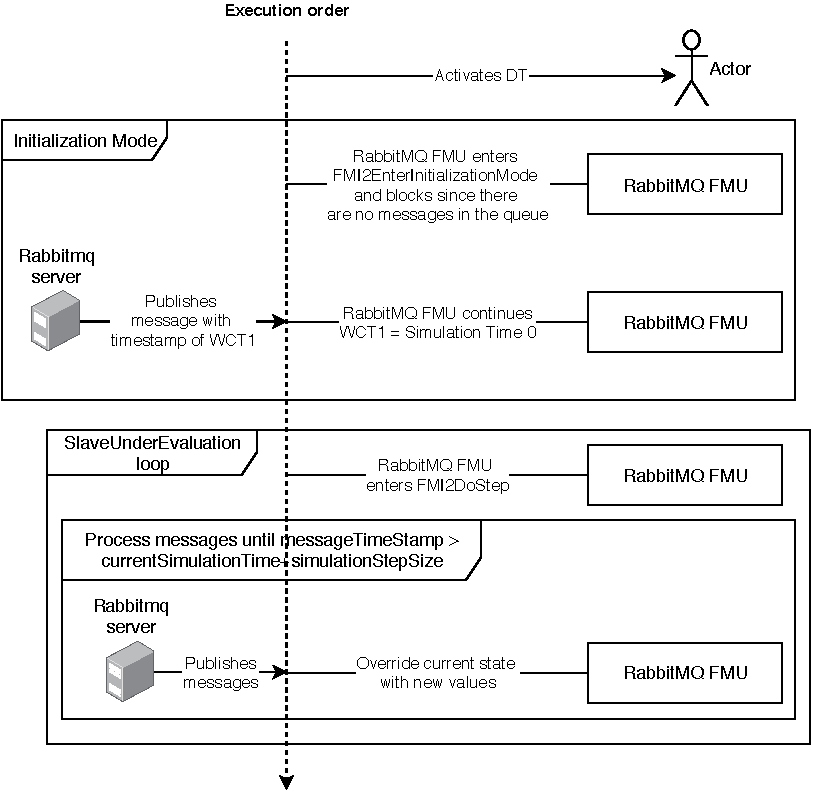
\includegraphics[width=\textwidth]{figures/timehandling.pdf}
  \caption{Time Handling in Simulation View}
  \label{fig:time-handling_simulation-view}
\end{figure}

Invoking the function \texttt{fmi2EnterInitializationMode} on EDB FMU causes it to
block until a message is available.\\
The time stamp of the first message ($WCT1$) received defines $simulationTime0$ and EDB
FMU continues. Thus $WCT1 = simulationTime0$ and a mapping between WCT and simulation time is
establishedcreated. Thus, any subsequent timestamps has $WCT1$ subtracted in order to map
them to $simulationTime$.\\
This also implies that any message with a time stamp of $WCT 0 < WCT1$ are ignored.

Invoking the function \texttt{fmi2DoStep} on EDB FMU causes it to process
messages and keep executing until there is a message with a time stamp defined by
$message\-TimeStamp\-InSimulationTime >= currentSimulationTime +
simulationStepSize$. Such a message is stored in order to use it for the
subsequent \texttt{fmi2DoStep} operation.

%%% Local Variables:
%%% mode: latex
%%% TeX-master: "../rabbitmq-fmu"
%%% End:

\newpage
\section{Data Handling}\label{sec:data_handling}
The data handling occurring within \texttt{fmi2DoStep} of EDB FMU is described
below.
All values of messages with time stamps (converted to simulation time) within the
time interval $]currentSimulationTime,currentSimulationTime + simulationStepSize]$
overrides the current state of values in the received order, thus using
zero-order hold. This depends on the Data Middleware Node providing the data
order by time, as mentioned in \cref{sec:intro}.

An example is given in \cref{fig:data-handling-dostep}.
First, \texttt{message x} is received and overwrites the value of \texttt{a} in the EDB FMU state.\\
Afterwards, \texttt{message y} is received and overwrites the value of \texttt{b} in
the EDB FMU state.\\
Lastly, \texttt{message z} is received and overwrites the value of
\texttt{a} in the EDB FMU state. \\
The example above implies that the value of \texttt{a} in \texttt{message x}  is never
outputted from the EDB FMU, since it has been overwritten by the value of
\texttt{a} in \texttt{message z} within the same \texttt{fmi2DoStep} execution.

\begin{figure}[htb]
  \centering
  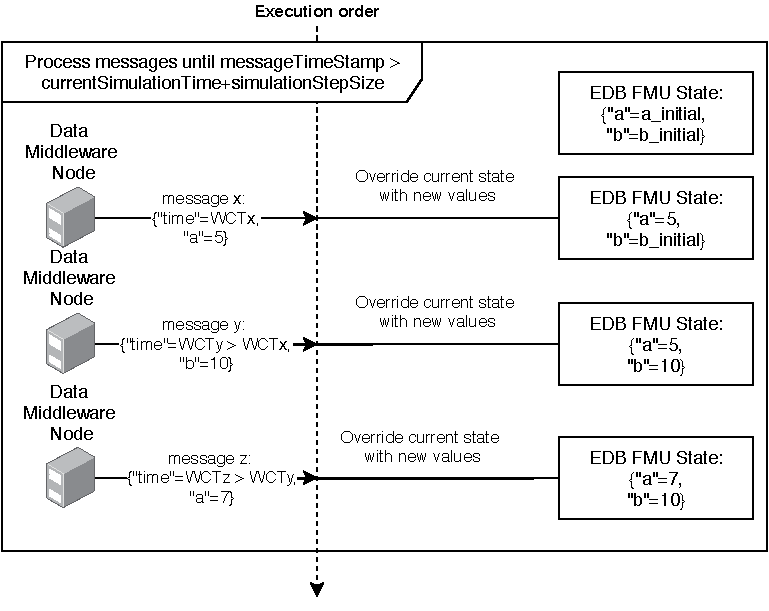
\includegraphics[width=\textwidth]{figures/datahandling.pdf}
  \caption{Data Handling in \texttt{fmi2DoStep}}
  \label{fig:data-handling-dostep}
\end{figure}

%%% Local Variables:
%%% mode: latex
%%% TeX-master: "../rabbitmq-fmu"
%%% End:

\clearpage
\section{Configuration}\label{sec:configuration}
This section covers how to configure an EDB FMU based on the RabbitMQ
implementation.
The data format of the messages is JavaScript Object Notation (JSON), which is
based on key/value pairs.

There are three key parts of the configuration: Configuring the data source connection,
configuring the behaviour of RabbitMQ FMU and
configuring the FMI outputs. The data source connection configuration specifies connection
details related to the RabbitMQ server. The behaviour configuration makes it
possible to alter quality attributes of RabbitMQ FMU. The FMI outputs configuration specifies which key/value pairs of the messages to
use.

This require changes to the FMU, but only to the static description file within
the FMU. Thus, the precompiled binary still works, since it parses the static
description file initially. Since RabbitMQ FMU has to parse the static
description file it is necessary to store a copy of the model description file
within the resources folder of the FMU.

\subsection{Configuring the Data Source Connection}
The data source connection is configured via FMI parameters, as these can be set externally
before \texttt{fmi2EnterInitializationMode}\footnote{This does not hold for all
  scalar variables with parameter as causality. Consult the FMI standard to ensure that you have the correct configuration.}. For this reason, it is possible to
either preconfigure the parameters in the static description file in the
resources folder of the FMU or set the values during execution of the FMU.

\Cref{lst:data-source-config} presents an example of configuring the data
source. Notice the combination of \texttt{causality="parameter"} and
\texttt{variability="fixed"} which implies that it is possible to set the values
before \texttt{fmi2EnterInitiali\-za\-tion\-Mode}, as it is necessary since a start
message is expected in the execution of \texttt{fmi2EnterInitializationMode} as
described in \cref{sec:time_handling}.
\lstset{
%  basicstyle=\ttfamily,
%  columns=fullflexible,
%  frame=single,
  postbreak=\raisebox{0ex}[0ex][0ex]
  {\ensuremath{\rcurvearrowse\space}},
  breakatwhitespace=true,
  breaklines=true,
  numbers=left,
  numberstyle=\scriptsize,
  frame=single
%  postbreak=\mbox{\textcolor{red}{$\hookrightarrow$}\space},
}
\begin{lstlisting}[label={lst:data-source-config},caption={Data source connection
    configuration of RabbitMQ FMU},language=XML]
<ScalarVariable name="config.hostname" valueReference="0" variability="fixed" causality="parameter">
    <String start="localhost"/>
</ScalarVariable>
<ScalarVariable name="config.port" valueReference="1" variability="fixed" causality="parameter">
    <Integer start="5672"/>
</ScalarVariable>
<ScalarVariable name="config.username" valueReference="2" variability="fixed" causality="parameter">
    <String start="guest"/>
</ScalarVariable>
<ScalarVariable name="config.password" valueReference="3" variability="fixed" causality="parameter">
    <String start="guest"/>
</ScalarVariable>
<ScalarVariable name="config.routingkey" valueReference="4" variability="fixed" causality="parameter">
    <String start="linefollower"/>
</ScalarVariable>
<ScalarVariable name="config.communicationtimeout" valueReference="6" variability="fixed" causality="parameter" description="Network read time out in seconds">
    <Integer start="60"/>
</ScalarVariable>
  \end{lstlisting}


\subsection{Configuring  FMI Outputs}
The scalar variables with \texttt{causality="output"} within the static
description are used by RabbitMQ FMU to define which key/value pairs to extract
from the messages that it receives. Thus, the name attribute of the output
scalar variable defines the key, whose paired value should be outputted as the
given scalar variable. Furthermore, the type of the value type must match the type of the
output scalar variable. An example is presented in \cref{lst:fmi-outputs-config}
where a single output of type \texttt{Real} is defined. Note, that the output
scalar variable must be added to the \texttt{Outputs} element based on index as
required by FMI, see \cref{lst:fmi-outputs-config2}. The name of the output scalar variable matches the
key/value pair \texttt{"level"} of a message such as the one exemplified in \cref{lst:message-example}

\begin{lstlisting}[label={lst:fmi-outputs-config},caption={FMI Outputs scalar
    variable configuration of RabbitMQ FMU},language=XML]
<!-- index=1 -->
<ScalarVariable name="level" valueReference="20" variability="continuous" causality="output">
    <Real />
</ScalarVariable>
\end{lstlisting}
\begin{lstlisting}[label={lst:fmi-outputs-config2},caption={FMI Outputs index
    configuration of RabbitMQ FMU },language=XML]
<Outputs>
    <Unknown index="1"/>
</Outputs>
\end{lstlisting}

\begin{lstlisting}[label={lst:message-example},caption={Example of a JSON message.},language=JSON]
{"time": 321, "level": 3.2}
  \end{lstlisting}

\subsection{Configuring Quality Attributes}
\label{subsec:cqa}
Precision is related to the communication step size passed to the function
\texttt{fmi2DoStep} of RabbitMQ FMU. See the description within the
\texttt{Scalar\-Variable} in \cref{lst:quality-attributes-config}.

\begin{lstlisting}[label={lst:quality-attributes-config},caption={Behaviour
configuration of RabbitMQ FMU},language=XML]
<ScalarVariable name="config.precision" valueReference="6" variability="fixed" causality="parameter" description="Communication step comparison precision. Number of decimals to consider" initial="exact">
    <Integer start="10"/>
</ScalarVariable>
  \end{lstlisting}

%%% Local Variables:
%%% mode: latex
%%% TeX-master: "../rabbitmq-fmu"
%%% End:

\clearpage
\section{Example Single Water Tank RabbitMQ}\label{sec:example-watertank}
The example in this section concerns a water tank with constant inflow and a
drain valve as depicted in \cref{fig:water-tank-picture}. The water level should
stay within a parameterised minimum and maximum water level. This is a brief
description, please see~\cite{INTOCPSD3.6} for additional information on
the models and co-simulation. Furthermore, historical data is passed in through
RabbitMQ FMU. \textbf{The entire example including a docker-compose file for
  starting a local RabbitMQ Node is available at \url{https://github.com/INTO-CPS-Association/example-single_watertank_rabbitmq}.}
\begin{figure}[!htb]
  \centering
  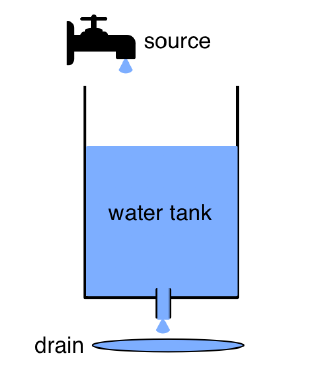
\includegraphics[]{figures/water-tank-picture.png}
  \caption{Water Tank}
  \label{fig:water-tank-picture}
\end{figure}

The example setup is shown in \cref{fig:rabbitmq-example} and consists of:
\begin{description}
  \item[Maestro] FMI Co-Simulation Engine
    \item[Tank FMU] Models the physical part of the water tank and outputs the
    water level within the tank. It receives the state of the drain valve as input.
    \item[Controller FMU] Models the controller of the drain valve. It outputs
    the state of the drain valve and receives the water level as input.
    Furthermore, it has the minimum water level and maximum water level as
    parameters
    \item[RabbitMQ Server] runs a RabbitMQ node.
  \item[Data] Contains historical water level data.
  \item[Python] Reads the data file and inputs it to RabbitMQ.
  \item[RabbitMQ FMU] Subscribes to RabbitMQ data.
    \item[Diff FMU] Only part of the co-simulation for technical issues related to plotting outputs.
\end{description}
\begin{figure}[!htb]
  \centering
  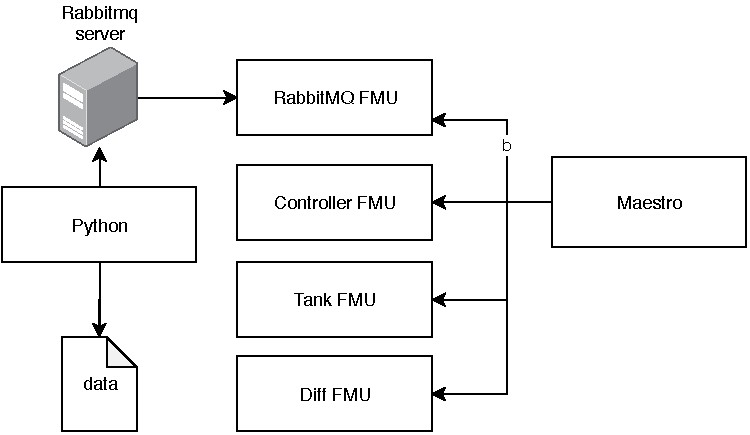
\includegraphics[]{figures/rabbitmq-example.pdf}
  \caption{Water Tank}
  \label{fig:rabbitmq-example}
\end{figure}

The result of executing the co-simulation is shown in TODO XX. The discrepancies
between the Tank FMU output and the RabbitMQ FMU output is related to
floating-point imprecision.



%%% Local Variables:
%%% mode: latex
%%% TeX-master: "../rabbitmq-fmu"
%%% End:

\clearpage
\section{Example Line Following Robot with Deployed System and RabbitMQ - IN PROGRESS}\label{sec:example-lfr}
The example in this section concerns a line following robot (LFR). An overview
of the example is presented in \cref{fig:lfr-example-overview}.

The deployed LFR publishes its sensor readings and actuator values to RabbitMQ
Node Queue 1. However, the deployed LFR is unaware of its position on the
track and the time. For this reason, a camera is used along with image recognition to detects its position. The
Log-Translator correlates the data from the deployed LFR and the
detection before publishing it to RabbitMQ Node Queue 2. As RabbitMQ FMU subscribes
to RabbitMQ Node Queue 2 it receives the messages. The
Controller FMU and the Physical FMU make up the models of the LFR, and the
modelled LFR is aware of its position on the track.

Thus, it is possible to realise the digital twin of the deployed LFR.


\textbf{The example including a docker-compose file for
  starting a local RabbitMQ Node is IN PROGRESS and you can follow it at
  \url{https://github.com/INTO-CPS-Association/example-DT-line_following_robot}.\\
See Issues in the repository for future work on the example.}
\begin{figure}[!htb]
  \centering
  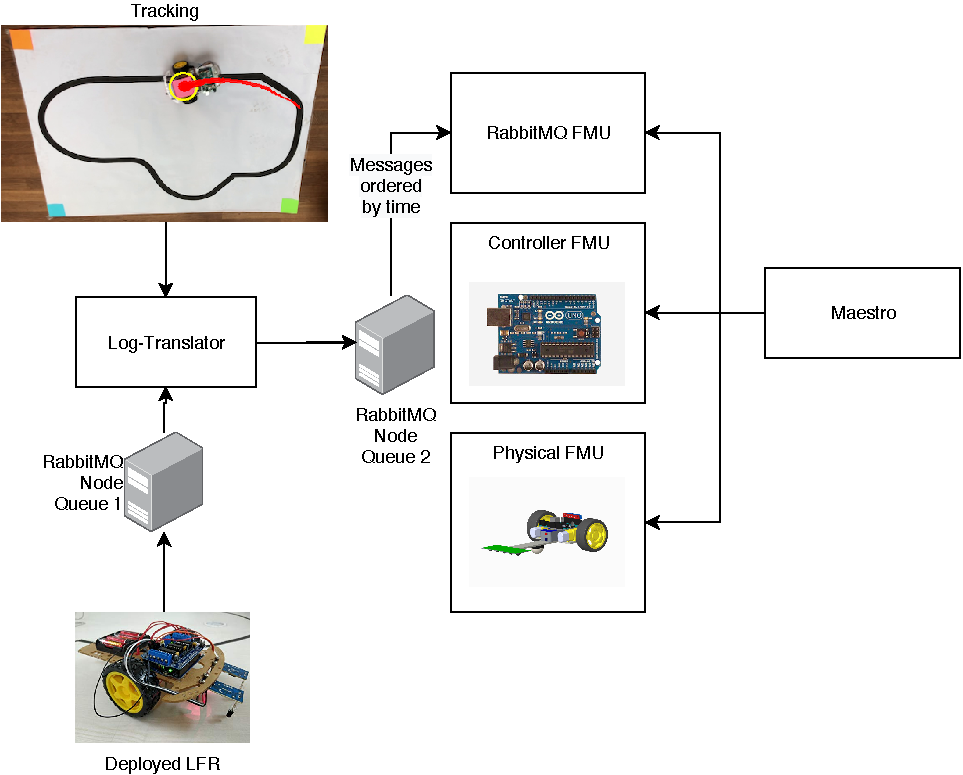
\includegraphics[width=\textwidth]{figures/lfr-example-overview.pdf}
  \caption{Water Tank}
  \label{fig:lfr-example-overview}
\end{figure}


%%% Local Variables:
%%% mode: latex
%%% TeX-master: "../rabbitmq-fmu"
%%% End:

\clearpage
\section{Future Work}\label{sec:future_work}
This section is not to be considered final and is subject to change in future revisions.

Some of the immediate future work is making the current research available at
the INTO-CPS Association github: \url{https://github.com/INTO-CPS-Association/}.

Other immediate future work is related to the LFR example, which was described
in \cref{sec:example-lfr}, and it is described at: \url{https://github.com/INTO-CPS-Association/example-DT-line_following_robot/issues}

%%% Local Variables:
%%% mode: latex
%%% TeX-master: "../rabbitmq-fmu"
%%% End:

%
%
%
%
%%%% Bibliography %%%%
\bibliographystyle{alpha}
\bibliography{bibliography}
\label{ch:bib} %label to refer to
%
%
%
\clearpage
%
%
%
\appendix
\section{List of Acronyms}\label{appendix:acronyms}
\begin{longtable}{ll}
XML	&Extensible Markup Language\\
\end{longtable}

\clearpage
%
%
%
\end{document}

%%% Local Variables:
%%% mode: latex
%%% TeX-master: t
%%% End:
